% Separate supplementary file for the Springer Nature submission package.
\documentclass[pdflatex,sn-mathphys-num,iicol]{sn-jnl}
\usepackage{graphicx}
\usepackage{multirow}
\usepackage{amsmath,amssymb}
\usepackage{booktabs}
\usepackage{tabularx}
\usepackage{url}
\usepackage{xurl}
\setlength{\emergencystretch}{3em}
\raggedbottom

\begin{document}

\title[Supplementary information]{Online Resource 1: Supplementary Information for ``Frozen Visual Representations for Relational Outfit Compatibility: A Leakage-Audited Cross-Dataset Study''}
\author*[1]{\fnm{Ali} \sur{Jamali}}\email{a.jamali2@salford.ac.uk}
\author[1]{\fnm{Maryam} \sur{Vadikheil}}
\author[1]{\fnm{Parham} \sur{Imanzadeh Charandabi}}
\author[1]{\fnm{Ali} \sur{Alameer}}
\author[1]{\fnm{Taha} \sur{Mansouri}}
\affil*[1]{\orgdiv{School of Science, Engineering and Environment}, \orgname{University of Salford}, \orgaddress{\city{Manchester}, \country{United Kingdom}}}
\maketitle

\noindent\textbf{Journal:} \emph{Machine Vision and Applications}

\section{Purpose and frozen evidence boundary}

This supplement expands the audit trail and robustness results without rerunning encoders or model training. Primary claims are based on Polyvore-D-Clean, the prospective IQON3000-Clean replication, and unchanged A100 evaluation. Historical Polyvore-D is retained only for literature-facing comparison. Post-audit diagnostics use frozen metadata, manifests, questions, and predictions and are explicitly identified below.

\section{Protocol construction details}

Polyvore-D-Clean is built from pooled historical positives after removing eight exact duplicate outfits. Exact file-byte and decoded-pixel hashes identify 120 duplicate-image groups. The outfit graph joins outfits sharing an item identifier or exact image group; entire connected components are assigned to one split. This yields 16,991/2,999/15,142 positive outfits and zero audited cross-split item, exact encoded-image, decoded-image, or outfit overlap.

IQON source validation starts from 308,747 JSON records. There are 297,916 valid outfits with at least two distinct items, 610 duplicate outfits, 3,568 users, and 712,170 unique source items. The largest item/image-connected component has 292,197 outfits (98.08\%), which makes a whole-component three-way split incompatible with useful evaluation sizes. The frozen balanced greedy hypergraph packing keeps identifiers and exact-image groups indivisible and discards boundary-conflicting outfits. Its exact targets are 86,800/12,400/24,800 outfits, or 41.62\% of valid outfits. This is an explicitly retained subset, not a claim to represent all IQON records.

Both clean datasets use one type- and length-aware corrupted outfit per positive for CP: every source item is replaced by a different same-category, within-split item. FITB uses one true item and three distinct same-category distractors drawn only from the same split, with candidate positions balanced. Seeds 42--46 vary these constructions while preserving the item partitions.

\subsection{Question-construction validity audit}

The builders reject generated CP item sets already present among observed positives, repeated generated negatives, FITB distractor completions that reproduce an observed positive, and duplicate candidates within a question. The post-audit validation traversed every frozen train/validation/test manifest and also compared decoded-pixel identities. In each of the six dataset--split combinations it found zero CP negative collisions with positives by item set, zero collisions by exact-image set, zero FITB duplicate candidate identifiers or exact images, and zero distractor completions equal to a known positive. CP negative counts equal positive counts and every negative item set is unique. Distractor reuse across different questions is permitted; its maximum multiplicity is one on Polyvore and two on IQON. These checks exclude exact false negatives and within-question duplication, not semantic false negatives or visually transformed copies.

\subsection{Historical-to-clean bridge}

\begin{table*}[t]
\caption{Historical packaged questions, historical positives with regenerated clean-style questions (bridge), and Polyvore-D-Clean. Values are CP ROC--AUC/FITB accuracy. The bridge isolates question construction approximately while retaining the historical positive split.}
\label{stab:bridge}
\centering\small
\begin{tabular}{lccc}
\toprule
Representation & Historical packaged & Historical regenerated & Clean \\
\midrule
ResNet50 & .6894/.4013 & .6945/.3975 & .6938/.4063 \\
DINOv3 & .7605/.4722 & .7839/.5024 & .7822/.5048 \\
CLIP & .8712/.6072 & .8876/.6394 & .8883/.6500 \\
SigLIP2 & .8729/.6224 & .8874/.6485 & .8892/.6528 \\
FashionCLIP & .8567/.5947 & .8699/.6197 & .8690/.6175 \\
Marqo & .8772/.6199 & .8891/.6440 & .8897/.6479 \\
GR-Lite & .8203/.5444 & .8216/.5490 & .8277/.5573 \\
\bottomrule
\end{tabular}
\end{table*}

Table~\ref{stab:bridge} shows that, across models, clean minus bridge ranges from $-0.0017$ to 0.0061 AUC and from $-0.0023$ to 0.0106 FITB. The larger packaged-to-regenerated changes show that absolute historical-to-clean movement is substantially affected by the regenerated CP negatives and FITB distractors. The bridge is not a perfect causal ablation because eight duplicate outfits and component assignments also differ in the final clean split; it nevertheless prevents the incorrect inference that leakage removal itself raised representation quality.

\subsection{IQON retained-subset and dependence audit}

\begin{table*}[t]
\caption{Post-audit comparison of retained and excluded valid IQON source outfits. Source-user activity and item frequency are computed from the full valid archive.}
\label{stab:iqonselection}
\centering\small
\begin{tabular}{lrr}
\toprule
Characteristic & Retained (124,000) & Excluded (173,916) \\
\midrule
Mean outfit length & 5.276 & 6.475 \\
Median outfit length & 5 & 6 \\
90th-percentile outfit length & 8 & 9 \\
Mean source-user activity & 283.19 & 302.57 \\
Median source-user activity & 292 & 336 \\
Mean item source frequency & 8.73 & 13.44 \\
Median within-outfit mean item frequency & 4.88 & 8.67 \\
Outfits containing a repeated item in source & 68.30\% & 80.88\% \\
\bottomrule
\end{tabular}
\end{table*}

The retained set contains 3,523 of 3,568 eligible users (98.74\%). Category-distribution divergence is small (Jensen--Shannon 0.0016 bits), whereas outfit-length divergence is larger (0.0190 bits) and the frequency summaries in Table~\ref{stab:iqonselection} reveal the selection mechanism's expected bias toward less-connected outfits. Users overlap substantially across the three retained splits, so this is not a user-disjoint test.

The IQON test-positive item graph has 9,231 connected components; its largest contains 11,547 of 24,800 outfits (46.56\%) and 7,245 are singletons. A 2,000-replicate paired component-cluster bootstrap using frozen predictions preserved every predefined contrast direction. Illustrative CP 95\% intervals are [0.0517,0.0651] for DINOv3--ResNet50, [0.0030,0.0154] for GR-Lite--DINOv3, [$-0.0105$,$-0.0003$] for FashionCLIP--CLIP, [0.0159,0.0257] for Marqo--SigLIP2, and [0.0140,0.0237] for Marqo--CLIP. Corresponding FITB intervals are [0.0434,0.0638], [0.0042,0.0227], [$-0.0157$,$-0.0008$], [0.0056,0.0200], and [0.0020,0.0171]. The sensitivity complements user clustering; because one component is large, it does not eliminate dependence uncertainty.

\section{Predefined statistical contrasts}

\begin{table*}[t]
\caption{Predefined clean-dataset contrasts. Effects are first minus second. CIs are 95\% paired, group-aware bootstrap intervals with 2,000 replicates. Holm correction is applied across the six comparisons within dataset--metric family. ``Supported'' means the adjusted test rejects at 0.05; it is not an equivalence statement for unsupported contrasts.}
\label{stab:effects}
\centering\small
\setlength{\tabcolsep}{2pt}\renewcommand{\arraystretch}{1.06}
\begin{tabularx}{\textwidth}{@{}>{\raggedright\arraybackslash}p{.23\textwidth}>{\centering\arraybackslash}p{.255\textwidth}>{\centering\arraybackslash}p{.255\textwidth}>{\raggedright\arraybackslash}X@{}}
\toprule
Contrast & CP AUC effect [CI] & FITB effect [CI] & Holm conclusion \\
\midrule
\multicolumn{4}{@{}l}{\textit{Polyvore-D-Clean}} \\
DINOv3 $-$ ResNet50 & .08845 [.08169,.09519] & .09853 [.08823,.10877] & both supported \\
GR-Lite $-$ DINOv3 & .04548 [.03994,.05113] & .05250 [.04246,.06195] & both supported \\
FashionCLIP $-$ CLIP & $-$.01935 [$-$.02319,$-$.01561] & $-$.03249 [$-$.04055,$-$.02384] & both supported \\
Marqo $-$ SigLIP2 & .00051 [$-$.00255,.00360] & $-$.00489 [$-$.01308,.00271] & neither supported \\
selected fashion $-$ generic & .00137 [$-$.00195,.00502] & $-$.00205 [$-$.01057,.00641] & neither supported \\
selected best $-$ ResNet50 & .19593 [.18988,.20177] & .24165 [.23161,.25122] & both supported \\
\midrule
\multicolumn{4}{@{}l}{\textit{IQON3000-Clean}} \\
DINOv3 $-$ ResNet50 & .05665 [.05077,.06259] & .04940 [.04165,.05805] & both supported \\
GR-Lite $-$ DINOv3 & .00920 [.00259,.01546] & .01718 [.00920,.02551] & both supported \\
FashionCLIP $-$ CLIP & $-$.00619 [$-$.01085,$-$.00150] & $-$.00891 [$-$.01590,$-$.00196] & both supported \\
Marqo $-$ SigLIP2 & .01904 [.01445,.02344] & .01206 [.00502,.01900] & both supported \\
selected fashion $-$ generic & .01790 [.01298,.02281] & .00867 [.00142,.01576] & both supported \\
selected best $-$ ResNet50 & .13691 [.13078,.14323] & .12847 [.12047,.13658] & both supported \\
\bottomrule
\end{tabularx}
\end{table*}

Table~\ref{stab:effects} reports the full predefined family. Polyvore CP resamples graph components and IQON resamples user clusters. FITB paired decisions use exact McNemar tests in the Polyvore analysis and paired bootstrap inference for effect sizes. A100 resamples questions. Practical-sensitivity reference levels, fixed before interpretation, are 0.002/0.005/0.010 for CP AUC, 0.5/1/2 percentage points for FITB, and 2/5/10 percentage points for A100.

\section{Calibration}

\begin{table*}[t]
\caption{CP probability quality. Lower Brier, log loss, and ECE are better; higher AUC is better. ECE is shown for 10, 15, and 20 equal-width bins to expose binning sensitivity.}
\label{stab:calibration}
\centering\small
\setlength{\tabcolsep}{5pt}\renewcommand{\arraystretch}{1.04}
\begin{tabular}{lrrrrrr}
\toprule
Representation & AUC & Brier & Log loss & ECE$_{10}$ & ECE$_{15}$ & ECE$_{20}$ \\
\midrule
\multicolumn{7}{l}{\textit{Polyvore-D-Clean}} \\
ResNet50 & .69375 & .22322 & .64508 & .02743 & .02884 & .02886 \\
DINOv3 & .78220 & .19158 & .59004 & .03188 & .03211 & .03275 \\
CLIP & .88830 & .13286 & .44702 & .03379 & .03407 & .03379 \\
SigLIP2 & .88917 & .13319 & .44729 & .03666 & .03724 & .03666 \\
FashionCLIP & .86896 & .14585 & .47607 & .03122 & .03046 & .03215 \\
Marqo & .88968 & .13218 & .44871 & .03423 & .03500 & .03423 \\
GR-Lite & .82768 & .16868 & .52837 & .03218 & .03490 & .03411 \\
\midrule
\multicolumn{7}{l}{\textit{IQON3000-Clean}} \\
ResNet50 & .58523 & .24989 & .69788 & .04017 & .04149 & .04032 \\
DINOv3 & .64188 & .24178 & .69496 & .04524 & .04623 & .04702 \\
CLIP & .70424 & .22610 & .68138 & .05532 & .05629 & .05687 \\
SigLIP2 & .70311 & .22643 & .68405 & .05386 & .05570 & .05587 \\
FashionCLIP & .69805 & .22808 & .68510 & .05725 & .05705 & .05738 \\
Marqo & .72214 & .21969 & .67022 & .05828 & .05825 & .05841 \\
GR-Lite & .65108 & .24024 & .69216 & .05691 & .05691 & .05691 \\
\bottomrule
\end{tabular}
\end{table*}

Table~\ref{stab:calibration} concerns binary CP probabilities under the constructed balanced 50:50 positive/negative protocol. Brier score, log loss, and ECE therefore measure benchmark calibration, not calibration to the unknown real-world prevalence of compatible outfits. FITB candidate scores are compared within a question and are not normalized probabilities, so ECE is not applied to FITB. The reliability diagrams in the main paper use the 15-bin definition.

\section{Representation-width and learner robustness}

\begin{table*}[t]
\caption{IQON PCA-256 versus native-dimensional features. Every native-width setting repeats train-only scaling and validation selection.}
\label{stab:native}
\centering\small
\resizebox{\textwidth}{!}{%
\begin{tabular}{lrrrrrr}
\toprule
Representation & PCA CP & Native CP & Difference & PCA FITB & Native FITB & Difference \\
\midrule
ResNet50 & .5852 & .6674 & .0821 & .3166 & .3644 & .0478 \\
DINOv3 & .6419 & .7144 & .0725 & .3660 & .4117 & .0456 \\
CLIP & .7042 & .7473 & .0431 & .4364 & .4440 & .0076 \\
SigLIP2 & .7031 & .7564 & .0533 & .4330 & .4649 & .0319 \\
FashionCLIP & .6981 & .7528 & .0547 & .4275 & .4606 & .0331 \\
Marqo & .7221 & .7593 & .0372 & .4451 & .4663 & .0213 \\
GR-Lite & .6511 & .6792 & .0281 & .3832 & .3953 & .0121 \\
\bottomrule
\end{tabular}}
\end{table*}

As Table~\ref{stab:native} shows, native features improve all point estimates. Rank agreement is nevertheless $\rho=0.857$, $\tau=0.714$ for CP and FITB. The choice of 256 dimensions is therefore consequential for absolute performance and computational normalization, but it does not create the broad hierarchy.

\begin{table*}[t]
\caption{IQON logistic versus XGBoost robustness over the same PCA-256 outfit features.}
\label{stab:xgb}
\centering\small
\resizebox{\textwidth}{!}{%
\begin{tabular}{lrrrr}
\toprule
Representation & Logistic CP & XGBoost CP & Logistic FITB & XGBoost FITB \\
\midrule
ResNet50 & .5852 & .5967 & .3166 & .3068 \\
DINOv3 & .6419 & .6564 & .3660 & .3390 \\
CLIP & .7042 & .7164 & .4364 & .3983 \\
SigLIP2 & .7031 & .7014 & .4330 & .3921 \\
FashionCLIP & .6981 & .7036 & .4275 & .3898 \\
Marqo & .7221 & .7265 & .4451 & .4055 \\
GR-Lite & .6511 & .6618 & .3832 & .3641 \\
\bottomrule
\end{tabular}}
\end{table*}

Table~\ref{stab:xgb} shows that CP rank agreement is $\rho=0.964$, $\tau=0.905$; FITB order is identical ($\rho=\tau=1$). The lower absolute XGBoost FITB values caution that a nonlinear CP learner is not automatically a better completion model.

\subsection{Compatibility-label efficiency}

The 10\%, 25\%, 50\%, and 100\% fractions reduce only labelled training outfits. Frozen encoders are unchanged, and PCA continues to use embeddings for every item in the full training split at all fractions. The outfit-feature StandardScaler and logistic classifier are refitted using the selected labelled outfits, with hyperparameter selection on validation CP. This analysis therefore estimates compatibility-label efficiency conditional on access to the full unlabeled training-item pool; it is neither generic low-data learning nor few-shot encoder adaptation.

\section{Construction and provenance sensitivity}

Across seeds 42--46, Polyvore CP Spearman agreement with the primary construction is 1.000, 1.000, 1.000, 0.893, and 1.000; FITB is 0.964 for every seed. IQON CP agreement is 1.000, 1.000, 0.964, 1.000, and 1.000; FITB is 1.000, 0.964, 0.964, 0.964, and 1.000. Standard deviations across constructions range from 0.00055 to 0.00206 for CP and 0.00122 to 0.00538 for FITB. These are measurement-construction effects, distinct from test-sample confidence intervals.

Removing Marqo-FashionSigLIP and GR-Lite leaves five checkpoints with no documented direct evaluation exposure, while still acknowledging possible web contamination. On Polyvore, SigLIP2 leads at 0.8892 CP and 0.6528 FITB; on IQON, CLIP leads at 0.7042 and 0.4364. FashionCLIP remains below CLIP on both datasets. Thus three conclusions survive the restriction: VLMs exceed ResNet50 and DINOv3, the broad hierarchy replicates, and fashion specialization is not universally beneficial. The full-roster statement that Marqo is strongest on IQON does not survive by definition and is always qualified by provenance.

\section{A100 label and facet sensitivity}

Each released LAT or AAT record supplies a partial outfit and five candidate items; each candidate is appended and the highest completed-outfit score is selected. LAT contains 847 reference instances, 680 referenced paths, and 680 unique exact images. AAT contains 983 reference instances and paths but 977 unique exact images. With 65 images shared between tasks, there are 1,663 referenced paths and 1,592 globally unique exact images. LAT primary accuracy uses the majority label $\arg\max$ of the released vote distribution. The nominal archive target differs on questions 92, 93, 94, 96, 98, 99, and 100. mLAT instead assigns the selected option its vote share. Polyvore-trained mLAT ranges from 0.330 (ResNet50) to 0.501 (Marqo); IQON-trained mLAT ranges from 0.234 to 0.474. The broad advantage of the evaluated VLM tier persists, while close-model ordering varies across accuracy, mLAT, and training source.

\begin{figure*}[t]
\centering
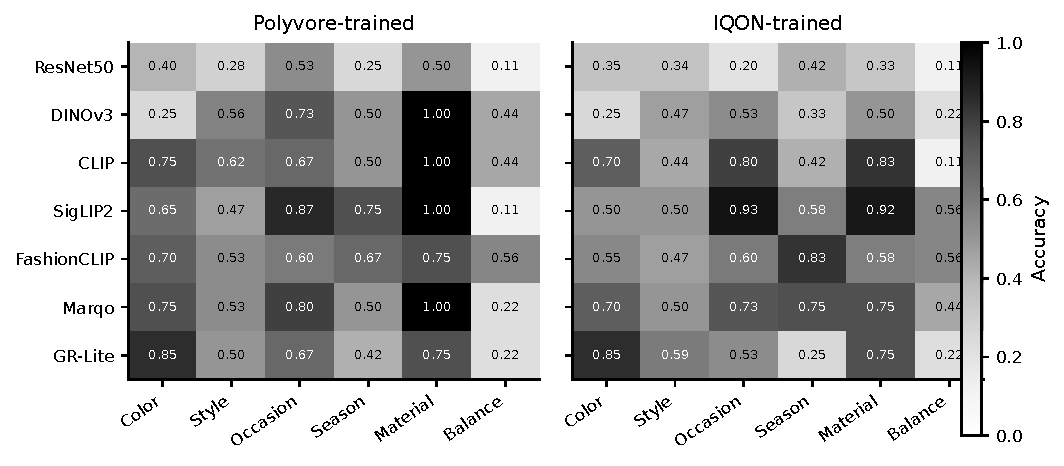
\includegraphics[width=0.93\textwidth]{figures/Fig9.pdf}
\caption{A100 AAT accuracy by released facet and training source. Facet sample sizes are colour 20, style 32, occasion 15, season 12, material 12, and balance 9; fine differences are correspondingly uncertain.}
\label{sfig:aat}
\end{figure*}

Figure~\ref{sfig:aat} is exploratory. The six facets have unequal and sometimes very small sample sizes, so it is inappropriate to use them as independent leaderboards. They are included to reveal whether an aggregate AAT value hides obvious dimension-specific failures.

\section{Retrieval overlap and failure consensus}

LookBench version~3 (revised 13 April 2026) has five exact checkpoint matches. Fine Recall@1 values are 43.97 (DINOv3), 39.79 (CLIP), 59.44 (SigLIP2), 62.77 (Marqo), and 65.71 (GR-Lite). Their Polyvore-D-Clean CP ranks are 5, 3, 2, 1, and 4, and FITB ranks are 5, 2, 1, 3, and 4; Spearman correlations are 0.20 and $-0.20$ (nominal $p=0.747$). IQON CP and FITB ranks are both 5, 2, 3, 1, and 4, yielding $\rho=0$ and $\tau=0$. Because $n=5$, these values document rank mismatch rather than establish population-level independence.

For CP, 463 of 30,284 Polyvore examples and 1,523 of 49,600 IQON examples are wrong for every frozen representation; 19,108 and 39,854, respectively, produce model disagreement. For FITB, the corresponding unanimous-error/disagreement counts are 965/12,089 of 15,142 and 3,497/20,200 of 24,800. Disagreement dominates consensus error, leaving scope for qualitative analysis or ensembles, but these counts do not by themselves identify causal failure modes.

\section{Reproducibility inventory}

\begin{table}[h!]
\caption{Frozen reproducibility identifiers.}
\label{stab:repro}
\centering\footnotesize
\begin{tabularx}{\columnwidth}{@{}>{\raggedright\arraybackslash}p{.24\columnwidth}>{\raggedright\arraybackslash}X@{}}
\toprule
Field & Frozen value \\
\midrule
Protocol & \texttt{repbench\_fashion\_final\_v1\_2} \\
Protocol SHA-256 & \texttt{96ffd69883c381f83a853ca6f73fbc30}\newline\texttt{cbd891366ba34f79ceb314cbe8d0f16b} \\
IQON split SHA-256 & \texttt{f5081ec5d2ea026216c126f370a54d27}\newline\texttt{cded601995f25904d3aed5bd6cde3f16} \\
Software & Python 3.12.13; PyTorch 2.11.0+cu128; Transformers 4.57.6; scikit-learn 1.9.1; CUDA 12.8 \\
Hardware & NVIDIA GeForce RTX 5070 Ti; Windows 11 \\
Artifact manifests & \texttt{artifacts/final\_artifact\_manifest.csv}; \texttt{artifacts/final\_report\_manifest.csv} \\
Version-control qualification & No initial Git commit existed at freeze; file and protocol hashes are the available provenance identifiers \\
\bottomrule
\end{tabularx}
\end{table}

Table~\ref{stab:repro} identifies the exact frozen protocol and software environment used for every reported result.

\end{document}
